\documentclass[a4paper,oneside]{ctexbook}
\usepackage{graphicx}
\usepackage{amsmath}
\usepackage{amssymb}
\usepackage{unicode-math}
\usepackage{cancel}
\usepackage{geometry}
\usepackage{amsfonts}
\usepackage{tikz}
\usepackage{caption}
\usepackage{booktabs}
\usepackage[toc]{multitoc}
\usepackage[colorlinks]{hyperref}
\geometry{a4paper,left=2.5cm,right=2.5cm,top=3cm,bottom=3cm}
\setlength{\headheight}{12.64723pt}
\addtolength{\topmargin}{-0.64723pt}
\setcounter{tocdepth}{1}
\linespread{1.8}\selectfont
\title{流体力学}
\author{***}
\date{期末复习资料}
\begin{document}

\frontmatter 

\maketitle

\chapter*{引言}

\section*{流体力学的研究对象和研究内容}


\subsection*{流体力学的基本内容}

流体力学是力学的一个分支,是研究水和空气之类的流体宏观运动规律,以及流体与固体之间相互作用和流体与流体之间的相互作用。
\begin{center}
    \begin{tabular}{|c|c|c|}
        \hline
        &流体 & 地球流体\\
        \hline
        液体 & 水 & 海洋\\
        \hline
        气体 & 空气 & 大气\\
        \hline
    \end{tabular}
\end{center}

\section*{研究方法(名称必背)}

理论方法,计算方法,实验方法。

\section*{应用}
\begin{enumerate}
    \item 航空,造船业外形设计操作性,稳定性。
    \item 水利工程水流对大坝的冲击力,水库,水电站的设计考虑洪峰极值。
    \item 气象科学研究大气运动的科学,自然离不开流体力学,流体力学是动力气象学,云雾动力学和边界层气象学的基础课。
    \item 海洋学研究海洋的运动规律。
    \item 天文学研究星云的气状物质运动等。
\end{enumerate} 

\tableofcontents

\mainmatter

\chapter{基础概念}

\section{物理性质(背)}

\subsection{流动性}

流体容易发生形变的特性。

\subsection{黏性}

抗切变性或阻碍流体的相对运动的特性。(黏性的存在与流体的运动有关,运动的黏性流体不一定显现出黏性)

液体的黏性随着温度的升高而减小(可根据水和冰来理解,冰的黏性大,温度低)气体的黏性随着温度的升高而增大(与液体相反)。

当流体的黏性很小,或相对速度不大时,流体的黏性力对流动的作用就不重要甚至可以略去,这种不考虑黏性的流体称为\textbf{理想流体}。

\subsection{压缩性}

流体的体积元在运动过程中可以因温度,压力等因素的改变而有所变化的特性。可分为可压缩流体和不可压缩流体。

\section{流体的连续介质假设--宏观理论模型}

把由离散分子构成的实际流体看成是无数流体质点没有间隙连续分布构成的,这就是流体连续介质假设。

注【1】微观足够大,统计时间足够长,碰撞次数足够多,流体分子的线尺度远远小于流体质点的线尺度,【2】宏观足够小流体质点的线尺度远远小于流体运动的线尺度。

\section{流体的速度和加速度}

\subsection{拉格朗日方法}

以流体质点的运动为研究对象,通过个别流点的运动特征得到整个流体运动特征。
\begin{enumerate}
    \item 流体中充满了流点,必须用数学方法把不同流点区分开来。 假定某一流点的初始时刻\(t\),位置位于点\((x_0,y_0,z_0)\)
    \item 考虑确定的参考系,取流点的位置矢径为\(\overrightarrow{r}\),且可以表示为\(\overrightarrow{r}=r(x_0,y_0,z_0,t)\)表示初始时刻\(t_0\)位置位于\((x_0,y_0,z_0)\)的流点,到\(t\)时,它们分别位于不同的位置。
\end{enumerate}

特别说明\((x_0,y_0,z_0)\)不是变量,只是用来区分不同的流点,\((x,y,z)\)才是位置变量,与\(t\)有关。

\subsection{欧拉方法(场的观点)}

着眼于空间点,由个别空间点运动特征得到整个流体运动特征。\(\overrightarrow{v}=v(x,y,z,t)\)不随\(t\)变化,表示流速在空间坐标点的分布,称作流速场或流场。

与流场有关的概念 

均匀流场:流场不随空间变化(速度在各个方向上梯度为0),反之则为非均匀流场。

定常流场:流场不随时间变化(对时间的偏微分为0),反之为非定常流场。

\subsection{两种变量之间的转换}

\subsubsection{拉格朗日变量转化为欧拉变量}

拉格朗日变量是描述单个流点的不同时刻的位置,而欧拉是空间固定点的速度,即对\(x,y,z\)求导,得到各点流速,在速度表达式中消去拉格朗日变量参数得到欧拉变量。

\subsubsection{欧拉变量转化为拉格朗日变量}

欧拉变量中速度为各个方向的导数,求积分即可得到拉格朗日变量。

\subsection{流体的加速度}

流体的加速度即为流速的时间变率。

对速度求导
\begin{equation}
    \dfrac{\mathrm{d}\overrightarrow{V}}{\mathrm{d}t}=\dfrac{\partial{}\overrightarrow{V}}{\partial{t}}+\dfrac{\partial{}\overrightarrow{V}\mathrm{d}x}{\partial{x}\mathrm{d}t}+\dfrac{\partial{}\overrightarrow{V}\mathrm{d}y}{\partial{y}\mathrm{d}t}+\dfrac{\partial{}\overrightarrow{V}\mathrm{d}z}{\partial{z}\mathrm{d}t}
\end{equation}

引入
\begin{equation}
    \nabla=\dfrac{\partial}{\partial{x}}\overrightarrow{i}+\dfrac{\partial}{\partial{y}}\overrightarrow{j}+\dfrac{\partial}{\partial{z}}\overrightarrow{k}
\end{equation}

有
\begin{equation}
    \dfrac{\mathrm{d}\overrightarrow{V}}{\mathrm{d}t}=\dfrac{\partial{\overrightarrow{V}}}{\partial{t}}+(\overrightarrow{V}\cdot\nabla)\overrightarrow{V}
\end{equation}
\begin{equation}(\overrightarrow{V}\cdot\nabla)=u\dfrac{\partial}{\partial{x}}+v\dfrac{\partial}{\partial{y}}+w\dfrac{\partial}{\partial{z}}\end{equation}
\begin{equation}\dfrac{\mathrm{d}(\ )}{\mathrm{d}t}=\dfrac{\partial{(\ )}}{\partial{t}}+(\overrightarrow{V}\cdot\nabla)(\ )\label{eqa1}\end{equation}

对于式\ref{eqa1}

左边第一项是\textbf{个别变化},流体质点在运动过程中物理量随时间的变化,

右边第一项是\textbf{局地变化},一固定空间点上物理量随时间的变化

右边第二项是\textbf{平流变化},反映了物理量场的非均匀性引起的变化。

\section{迹线和流线}

\subsection{迹线}

某个流点在各时刻所行路径的轨迹线,或者说是流体质点运动的轨迹线。它描绘了某一确定流点在不同时刻所处的空间位置和运动方向,消去\(t\)即可求得。

\subsection{流线}

在某一固定时刻,曲线上的任意一点流速方向与该点切线方向相吻合,这样的曲线称为流线

注意:流线只反映流速方向,不能反映流速大小。由流线形成的管状曲面称为流管,流管不能相交。

求流线方程时,假设\(\mathrm{d}\overrightarrow{r}\)为流线的线元矢量,其可以表示为\(\mathrm{d}\overrightarrow{r}=\mathrm{d}x\overrightarrow{i}+\mathrm{d}y\overrightarrow{j}+\mathrm{d}z\overrightarrow{k}\)根据流线的定义和矢量积的性质,流线的微分方程\(\mathrm{d}\overrightarrow{r}\times\overrightarrow{V}=0\),即
\begin{equation}
    \dfrac{\mathrm{d}x}{u(x,y,z,t)}=\dfrac{\mathrm{d}y}{v(x,y,z,t)}=\dfrac{\mathrm{d}z}{w(x,y,z,t)}
\end{equation}

积分上式即可。

几个易混概念
\begin{enumerate}
    \item 定常流场迹线和流线一定重合\((\checkmark)\)
    \item 迹线和流线重合,则为定常流场\((\times)\quad(u=at,v=0,w=0)\)
    \item 定常流动,流线不随时间变变化\((\checkmark)\)
    \item 流线随时间不变,则为定常流动\((\times)\quad{}u=aty,v=atx,w=0\)
    \item 稳定流场流线不随时间变化\((\checkmark)\)
    \item 流线不随时间变化,流场为稳定流场\((\times)\)
\end{enumerate}

\section{速度分解}

\subsection{亥姆霍兹速度分解定理}

流体微团的运动可分解为平动速度\(\overrightarrow{V}_O\)转动线速度\(\overrightarrow{V}_R\)和形变线速度\(\overrightarrow{V}_D\)三部分。\begin{equation}\overrightarrow{V}_D=A\cdot\delta\overrightarrow{r}\end{equation}

定义形变张量\(A\)
\begin{equation}
A=\begin{pmatrix}
    e_{11}&e_{12}&e_{13}\\
    e_{21}&e_{22}&e_{23}\\
    e_{31}&e_{32}&e_{33}\\
\end{pmatrix}
\end{equation}

其中切形变率
\begin{equation}
    \begin{cases}
    e_{12}=e_{21}=\dfrac{1}{2}(\dfrac{\partial{v}}{\partial{x}}+\dfrac{\partial{u}}{\partial{y}})\\
    e_{31}=e_{31}=\dfrac{1}{2}(\dfrac{\partial{w}}{\partial{x}}+\dfrac{\partial{u}}{\partial{z}})\\
    e_{23}=e_{32}=\dfrac{1}{2}(\dfrac{\partial{w}}{\partial{y}}+\dfrac{\partial{v}}{\partial{z}})\\
    \end{cases}
\end{equation}

公式的记忆方法就是下标对应方向的位置与速度偏微分重组

法形变率
\begin{equation}
    \begin{cases}
    e_{11}=\dfrac{\partial{u}}{\partial{x}}\\
    e_{22}=\dfrac{\partial{v}}{\partial{y}}\\
    e_{33}=\dfrac{\partial{w}}{\partial{z}}
    \end{cases}
\end{equation}
\begin{equation}
\overrightarrow{V}_R=\overrightarrow{\omega}\times\delta\overrightarrow{r}
\end{equation}
\begin{equation}
\overrightarrow{\omega}=\dfrac{1}{2}\nabla\cdot\overrightarrow{V}=\dfrac{1}{2}\left[\left(\dfrac{\partial{v}}{\partial{x}}-\dfrac{\partial{u}}{\partial{y}}\right)\overrightarrow{k}+\left(\dfrac{\partial{u}}{\partial{z}}-\dfrac{\partial{w}}{\partial{x}}\right)\overrightarrow{j}+\left(\dfrac{\partial{w}}{\partial{y}}-\dfrac{\partial{v}}{\partial{z}}\right)\overrightarrow{i}\right]
\end{equation}

\section{散度和涡度}

\subsection{散度定义为\(\nabla\cdot\overrightarrow{V}\)}

物理意义:单位体积的流体通量

由奥高公式推到\(\nabla\cdot\overrightarrow{V}=\lim_{\tau\to0}\limits\dfrac{F}{\tau},\quad{}F=\oiint_\sigma\overrightarrow{V}\cdot\overrightarrow{n}\delta\sigma\)(流体通量)

\(\nabla\cdot\overrightarrow{V}>0\),流体净流出,源(辐散)

\(\nabla\cdot\overrightarrow{V}<0\),流体净流入,汇(辐合)

度量流体体积膨胀或收缩的一个量,单位体积的体积胀率

体形变\(\nabla\cdot\overrightarrow{V}=\dfrac{\mathrm{d}(\delta\tau)}{\mathrm{d}t}\)

\subsection{旋度(涡度)定义为\(\nabla\times\overrightarrow{V}\)}

物理意义:度量旋转流体旋转程度的物理量。

速度环流在流体中取一个闭合有向曲线,沿闭合曲线\(l\)对该曲线流速积分求和,即\(\Gamma=\oint_l\overrightarrow{V}\cdot\mathrm{d}l\),表示闭合流体运动趋势的程度

由公式\(\Gamma=\oint_l\overrightarrow{V}\cdot\mathrm{d}l=\oiint_\sigma\nabla\times\overrightarrow{V}\delta\sigma\),面积无限趋于0,有\(\nabla\times\overrightarrow{V}\cdot\overrightarrow{n}=\lim_{\sigma\to0}\limits\dfrac{\Gamma}{\sigma}\),即流体某点涡度矢在单位面元上的法向分量为单位面积速度环流的极限值。

流体的涡度是自转不是公转。

\section{速度流函数和势函数}

\subsection{无旋流动必然存在势函数。}

如果在流体域内涡度为零,即\(\nabla\times\overrightarrow{V}=0\)(无旋流动)否则,则称之为涡旋流动\(\nabla\times\overrightarrow{V}\ne0\)

据矢量分析知识,任意一函数的梯度取旋度恒等于零\begin{equation}\nabla\times(-\nabla\varphi)=0\end{equation}

对于无旋流动,必定存在一个函数\(\varphi(x,y,z,t)\)满足\begin{equation}\overrightarrow{V}=-\nabla\varphi\end{equation}

\subsection{无旋流动}

\textbf{其速度矢可以用某函数\(\varphi\)的梯度来表示,把函数\(\varphi(x,y,z,t)\)叫做速度的位势函数,可以用这个函数来表示无旋流动的流场。}

势函数与速度矢的关系
\begin{gather*}
    \overrightarrow{V}=u\overrightarrow{i}+v\overrightarrow{j}+w\overrightarrow{k}\\
    \overrightarrow{V}_\varphi=\dfrac{\partial\varphi}{\partial{x}}\overrightarrow{i}+\dfrac{\partial\varphi}{\partial{y}}\overrightarrow{j}+\dfrac{\partial\varphi}{\partial{z}}\overrightarrow{k}\\
    \overrightarrow{V}=-\nabla\varphi\\
    u=-\dfrac{\partial\varphi}{\partial{x}}\quad v=-\dfrac{\partial\varphi}{\partial{y}}\quad w=-\dfrac{\partial\varphi}{\partial{z}}
\end{gather*}

势函数优点只要一个变量(势函数)就可以来描述流体运动,减少了描写流体运动所需的变量,从而简化问题,另一个好处就是可以用速度势来表征流体散度。

势函数可以类比于电场强度和电势的关系,电场为有源无旋场,所以存在势函数电势。\(\varphi=C\),即为等势面由流速场与势函数的关系可知\(\overrightarrow{V}=-\nabla\varphi\)

\subsection{流函数\(\psi(x,y,t)\)二维无辐散}

\(P\mathrm{d}x+Q\mathrm{d}y\)可以写成某一个函数\(F\)的全微分的话,充要条件是\(\dfrac{\partial{P}}{\partial{y}}=\dfrac{\partial{Q}}{\partial{x}}\)

与无辐散运动很像\(\dfrac{\partial{v}}{\partial{y}}=-\dfrac{\partial{u}}{\partial{x}}\)

也就是说由无辐散条件,就可以找到一个函数与速度矢对应,我们把这个函数写成\(\psi\)
\begin{equation}
    \mathrm{d}\psi(x,y,z)=v(x,y,z)\mathrm{d}x-u(x,y,z)\mathrm{d}y
\end{equation}

流速与该函数满足\(u=-\dfrac{\partial\psi}{\partial{y}},v=\dfrac{\partial\psi}{\partial{x}}\)

矢量形式\(\overrightarrow{V}=\overrightarrow{k}\times\nabla\psi\)

令\(\mathrm{d}\psi(x,y,t)=0\)对\(\mathrm{d}\psi(x,y,t)=v(x,y,t)\mathrm{d}x-u(x,y,t)\mathrm{d}y\)积分,得
\begin{equation}
    \psi(x,y,t)=const
\end{equation}

上式时间确定,常数也取定时,就代表了某时刻的某一条流线,或等流函数线,此曲线上的切线处处跟流速矢方向一致。

流函数也可以用来表征流体涡度
\begin{equation}
    \dfrac{\partial^2\psi}{\partial{x^2}}+\dfrac{\partial^2\psi}{\partial{y^2}}=\xi
\end{equation}

流函数图像就是流线,流线越密流速越大,流速方向垂直等势线,由高值指向低值。

注【1】流速矢与等位势面相垂直。【2】由高位势流向低位势。【3】等位势面紧密处,位势梯度大。相应的流速大,等位势面稀疏处,位势梯度小,相应的流速小。无旋必有势,有势必无旋。

\section{总结散度旋度以及流函数,势函数}

\subsection{rot 涡度\(\nabla\times\overrightarrow{V}\)}

速度环流
\begin{equation}
    \Gamma=\oint_l\overrightarrow{V}\cdot\mathrm{d}\overrightarrow{l}=\oiint_\sigma\nabla\times\overrightarrow{V}\cdot\mathrm{d}\overrightarrow{\sigma}
\end{equation}

由
\begin{equation}
    \lim_{\sigma\to0}\left[\dfrac{\oiint_\sigma\nabla\times\overrightarrow{V}\mathrm{d}\overrightarrow{\sigma}}{\iint_\sigma\mathrm{d}\overrightarrow{\sigma}}\right]=\lim_{\sigma\to0}\dfrac{\Gamma}{\sigma}=\nabla\times\overrightarrow{V}\cdot\overrightarrow{n}
\end{equation}

可以得到流点的涡度在单位面积的法向分量与单位面积速度环流的极限值相等。

在\(z\)方向上
\begin{equation}
\left(\nabla\times\overrightarrow{V}\right)_z=\left(\nabla\times\overrightarrow{V}\right)_k=\left(\dfrac{\partial{v}}{\partial{x}}-\dfrac{\partial{u}}{\partial{y}}\right)
\begin{pmatrix}
\overrightarrow{i}&\overrightarrow{j}&\overrightarrow{k}\\
\dfrac{\partial}{\partial{x}}&\dfrac{\partial}{\partial{y}}&\dfrac{\partial}{\partial{z}}\\
u&v&w\\
\end{pmatrix}
\end{equation}

若\(w=0,\dfrac{\partial{v}}{\partial{x}}=-\dfrac{\partial{u}}{\partial{y}}\)即旋转角速度为
\begin{equation}
    2\overrightarrow{\omega}=\nabla\times\overrightarrow{V}
\end{equation}

\subsection{div 散度\(\nabla\cdot\overrightarrow{V}\)}

由体积通量\(F=\iint_{\sigma}\overrightarrow{V}\cdot\mathrm{d}\overrightarrow{\sigma}=\iiint_\tau\nabla\cdot\overrightarrow{V}\mathrm{d}\tau\),对其取单位体积的极限
\begin{equation}
    \lim_{\tau\to0}\left[\dfrac{\iiint_\tau\nabla\cdot\overrightarrow{V}\mathrm{d}\tau}{\iiint_\tau\mathrm{d}\tau}\right]=\lim_{\tau\to0}\dfrac{F}{\tau}=\nabla\cdot\overrightarrow{V}
\end{equation}

可以得知散度为单位体积的体积通量。
\begin{equation}
\left\{
    \begin{array}{l l}
    \nabla\cdot\overrightarrow{V}>0&\text{体积膨胀,源}\\
    \nabla\cdot\overrightarrow{V}<0&\text{体积收缩,汇}
    \end{array}
\right.
\end{equation}

同时,散度还可以用法形变之和,单位体积的体胀速度来表示。

\subsection{势函数(运动的有无旋)}

已知\(\nabla\times\nabla\varphi\equiv0\),对于无旋运动而言,\(\nabla\times\overrightarrow{V}=0\),即存在\(\varphi\),使得\(\overrightarrow{V}=-\nabla\varphi\)

等势面\(\varphi=C\)(\(C\)为任意常数)
\begin{equation}
    D=\dfrac{\partial{u}}{\partial{x}}+\dfrac{\partial{v}}{\partial{y}}+\dfrac{\partial{w}}{\partial{z}}
\end{equation}

将
\begin{equation}
\left\{
\begin{array}{c}
    u=-\dfrac{\partial{\varphi}}{\partial{x}}\\
    v=-\dfrac{\partial{\varphi}}{\partial{y}}\\
    w=-\dfrac{\partial{\varphi}}{\partial{z}}\\
\end{array}
\right.
\end{equation}

代入可得
\begin{equation}
    \dfrac{\partial^2\varphi}{\partial{x^2}}+\dfrac{\partial^2\varphi}{\partial{y^2}}+\dfrac{\partial^2\varphi}{\partial{z^2}}=-D
\end{equation}

即
\begin{equation}
    \nabla^2\varphi=-D
\end{equation}

\subsection{流函数(运动的有无辐散)}

对于二维无辐散运动
\begin{equation}
\left\{
\begin{array}{l}
    w=0\\
    u=u(x,y,z),v=v(x,y,z)\\
    u_x+v_y=0\\
\end{array}
\right.
\end{equation}

流线方程
\begin{equation}
    \dfrac{\mathrm{d}x}{u}=\dfrac{\mathrm{d}y}{v}
\end{equation}

即
\begin{equation}
    v\mathrm{d}x-u\mathrm{d}y=0
\end{equation}

流线为等流函数线
\begin{equation}
    \Psi=C
\end{equation}

\(C\)为任意常数

改写为全微分形式
\begin{equation}
\mathrm{d}\varphi(x,y,t)=vdx-udy=0\quad
\left\{
\begin{array}{l}
    u=-\dfrac{\partial{\psi}}{\partial{y}}\\
    v=\dfrac{\partial{\psi}}{\partial{x}}\\
\end{array}
\right.
\end{equation}

由涡度
\begin{equation}
    \overrightarrow{\zeta}=\dfrac{\partial{v}}{\partial{x}}-\dfrac{\partial{u}}{\partial{y}}
\end{equation}

可得流函数
\begin{equation}
    \dfrac{\partial^2\psi}{\partial{x^2}}+\dfrac{\partial^2\psi}{\partial{y^2}}=\overrightarrow{\zeta}
\end{equation}

总结

求加速度
\begin{equation}
\begin{array}{c}
    a_x=\dfrac{\partial{u}}{\partial{t}}+u\dfrac{\partial{u}}{\partial{x}}+v\dfrac{\partial{u}}{\partial{y}}+w\dfrac{\partial{u}}{\partial{z}}\\
    a_y=\dfrac{\partial{v}}{\partial{t}}+u\dfrac{\partial{v}}{\partial{x}}+v\dfrac{\partial{v}}{\partial{y}}+w\dfrac{\partial{v}}{\partial{z}}\\
    a_z=\dfrac{\partial{w}}{\partial{t}}+u\dfrac{\partial{w}}{\partial{x}}+v\dfrac{\partial{w}}{\partial{y}}+w\dfrac{\partial{w}}{\partial{z}}\\
\end{array}
\end{equation}

求流线方程
\begin{equation}
    \dfrac{\mathrm{d}x}{u}=\dfrac{\mathrm{d}y}{v}
\end{equation}

\chapter{流体运动的控制方程}

两种连续方程之间的不同和推导,散度的物理意义,平流项的意义

\section{流体的连续方程}

\subsection{拉格朗日连续方程}
\begin{figure}[htbp]
    \centering
    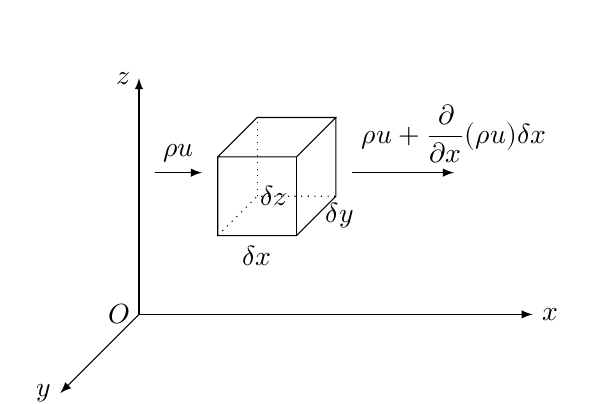
\begin{tikzpicture}[>=latex]
        \draw[->] (0,0)node[left]{\(O\)}--(-1,-1)node[left]{\(y\)};
        \draw[->] (0,0)--(0,3)node[left]{\(z\)};
        \draw[->] (0,0)--(5,0)node[right]{\(x\)};
        \draw (1,2)--(1.5,2.5)--(2.5,2.5)--(2,2)--(1,2)--(1,1)--node[below]{\(\delta x\)}(2,1)--node[right]{\(\delta y\)}(2.5,1.5)--(2.5,2.5);
        \draw (2,1)--node[left]{\(\delta z\)}(2,2);
        \draw[dotted] (1,1)--(1.5,1.5)--(2.5,1.5);
        \draw[dotted] (1.5,1.5)--(1.5,2.5);
        \draw[->] (0.2,1.8)--node[above]{\(\rho u\)}(0.8,1.8);
        \draw[->] (2.7,1.8)--(4,1.8)node[above]{\(\rho u+\dfrac{\partial}{\partial{x}}(\rho u)\delta x\)};
    \end{tikzpicture}
    \caption{流体连续性}
\end{figure}
\begin{equation}\Delta{v}=\Delta{x}\Delta{y}\Delta{z}\end{equation}

由质量守恒可以推出拆成
\begin{equation}
    \Delta{m}=\rho\Delta{v}\quad\dfrac{\mathrm{d}\Delta{m}}{\mathrm{d}\Delta{t}}=\dfrac{\mathrm{d}(\rho\Delta{v})}{\mathrm{d}t}=0
\end{equation}

微分形式,即
\begin{equation}
    \rho\dfrac{\mathrm{d}\Delta{v}}{\mathrm{d}t}+\Delta{v}\dfrac{\mathrm{d}\rho}{\mathrm{d}t}=0
\end{equation}

两边同时除以\(\rho\Delta{v}\)
\begin{equation}
    \dfrac{\mathrm{d}\rho}{\rho\mathrm{d}t}+\dfrac{\mathrm{d}\Delta{v}}{\Delta{v}\mathrm{d}t}=0
\end{equation}

第一项相对密度变化率(个别变化率)

第二项流速的变化(体积变化)
\begin{equation}
    \dfrac{\mathrm{d}\rho}{\mathrm{d}t}+\rho\nabla\cdot\overrightarrow{V}=0
\end{equation}

拉氏观点的连续方程,它表明流速分布必须与密度变化按连续方程相互约束,否则将破坏流体的连续介质假定。
\begin{enumerate}
    \item \(\nabla\cdot\overrightarrow{V}>0\Rightarrow\)流体体积增大\(\Rightarrow\dfrac{\mathrm{d}\rho}{\mathrm{d}t}<0\Leftrightarrow\)流体密度减小,
    \item \(\nabla\cdot\overrightarrow{V}<0\Rightarrow\)流体体积减小\(\Rightarrow\dfrac{\mathrm{d}\rho}{\mathrm{d}t}>0\Leftrightarrow\)流体密度增大,
    \item \(\nabla\cdot\overrightarrow{V}=0\Rightarrow\)流体体积不变\(\Rightarrow\dfrac{\mathrm{d}\rho}{\mathrm{d}t}=0\Leftrightarrow\)流体密度不变,
\end{enumerate}

\subsection{欧拉连续方程}

由拉格郎日型连续方程推导欧拉型连续方程
\begin{gather}
    \dfrac{\mathrm{d}\rho}{\mathrm{d}t}+\rho\nabla\cdot\overrightarrow{V}=0\\
    \dfrac{\mathrm{d}\rho}{\mathrm{d}t}=\dfrac{\partial{\rho}}{\partial{t}}+\overrightarrow{V}\cdot\nabla\rho
\end{gather}

所以
\begin{equation}
    \dfrac{\partial{\rho}}{\partial{t}}+\nabla\cdot(\rho\overrightarrow{V})=0
\end{equation}

欧拉观点的连续方程,空间某点流体质量有净外流时,密度减少,反之。流动改变了流体质量的分布

公式改写\(\dfrac{\partial{\rho}}{\partial{t}}=-\nabla\cdot(\rho\overrightarrow{V})\)

\(\dfrac{\partial{\rho}}{\partial{t}}\)流体密度的局地变化

\(\nabla\cdot(\rho\overrightarrow{V})\)单位体积的流体质量通量
\begin{enumerate}
    \item \(\nabla\cdot\rho\overrightarrow{V}>0\Rightarrow\)流体有净流出\(\Rightarrow\dfrac{\partial{\rho}}{\partial{t}}<0\Leftrightarrow\)流体局地密度减小
    \item \(\nabla\cdot\rho\overrightarrow{V}<0\Rightarrow\)流体有净流入\(\Rightarrow\dfrac{\partial{\rho}}{\partial{t}}>0\Leftrightarrow\)流体局地密度增大,
    \item \(\nabla\cdot\rho\overrightarrow{V}=0\Rightarrow\)流体出入平衡\(\Rightarrow\dfrac{\partial{\rho}}{\partial{t}}=0\Leftrightarrow\)流体局地密度不变
\end{enumerate}

流动改变了流体质量的分布

\subsection{自由表面的流体连续方程,在第四章会用到}

设流体自由表面高度\(h=h(x,y,t)\),即\(h\)在各处不同且随\(t\)变化(与欧拉方程的推导相似)\(\dfrac{\partial{h}}{\partial{t}}+\nabla\cdot(h\overrightarrow{V})=0\)
\begin{equation}
    \dfrac{\mathrm{d}\rho}{\mathrm{d}t}=\dfrac{\partial{\rho}}{\partial{t}}+\overrightarrow{V}\cdot\nabla\rho=0
\end{equation}

表示流体质点在运动中密度不变,但\(\dfrac{\partial{\rho}}{\partial{t}}\)和\(\overrightarrow{V}\cdot\nabla\rho\)不一定为零

\(\overrightarrow{V}\cdot\nabla\rho\)密度的不均匀性 \(\nabla\rho=0\)密度在空间处处都一样
\begin{enumerate}
    \item \(\dfrac{\partial{\rho}}{\partial{t}}\neq0\)不定常
    \item \(\dfrac{\partial{\rho}}{\partial{t}}=0\)流体定常
    \item \(\dfrac{\mathrm{d}\rho}{\mathrm{d}t}=0\)流体质点在运动中密度不变,流场中的流体密度可以是不定常和不均匀的,只要两者的变化对流体块的贡献正好抵消就可以
    \item \(\nabla\rho=0\)均质流体。 流体密度空间处处相等,但可能随时间在变化
    \item \(\dfrac{\mathrm{d}\rho}{\mathrm{d}t}=0\)或\(\nabla\cdot\overrightarrow{V}=0\)不可压缩流体。某一流体质点在运动中保持密度不变,但各个空间上的密度可能不同
    \item \(\dfrac{\mathrm{d}\rho}{\mathrm{d}t}=0\)且\(\nabla\rho=0\)均匀不可压缩流体。密度不但在空间处处相等,而且在运动中保持不变。均匀不可压缩流体也叫定常不可压流体
    \item \(\dfrac{\mathrm{d}\rho}{\mathrm{d}t}=0\)且\(\nabla\rho\neq0\)非均匀不可压缩流体。密度在空间上分布是不均匀的,但在运动中始终保持这种分布
\end{enumerate}

\section{表面应力}

\subsection{质量力(可能会考)}

定义:作用于所有流体质点的力,与周围的流点无关。

F表示单位质量的流体的质量力\(F=\lim_{\delta{m}\to0}\limits\dfrac{\delta{F}'}{\delta{m}}\)

常见的有重力,万有引力等。

通常情况下,作用于流体的质量力通常就是指重力。

属于长程力,通常用F来表示质量力分布密度,它是时间点和空间点的函数。

\subsection{表面力}

定义:直接接触而作用于流体界面上的力

单位面积上的表面力为\(\overrightarrow{p}=\lim_{\delta\sigma\to0}\limits\dfrac{\delta{p}}{\delta\sigma}\),其\(\overrightarrow{p}\)是作用于某个流体面积上的表面力。

流体内各部分之间,或流体与固体之间通过邻接表面的相互作用力均属表面力。

属于短程力,它不但是时间和空间点的函数,并且在空间每一点还随着受力面元的取向不同而变化

\subsection{应力张量}
\begin{equation}
P=\begin{pmatrix}
    p_{xx}&p_{xy}&p_{xz}\\
    p_{yx}&p_{yy}&p_{yz}\\
    p_{zx}&p_{zy}&p_{zz}\\
\end{pmatrix}
\end{equation}

应力张量的9个分量中,\(p_{xx},p_{yy},p_{zz}\)称为法应力(是\(YOZ\)平面,\(XOZ\)平面,\(XOY\)平面法向上的分量)。其余6个量称为切应力(分量)
\begin{figure}[htbp]
    \centering
    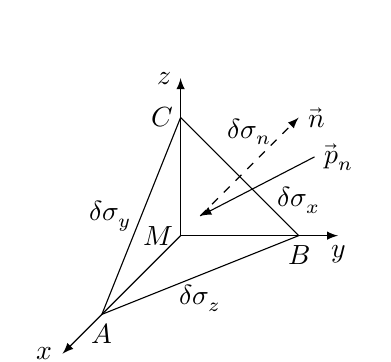
\begin{tikzpicture}[>=latex]
        \draw[->] (0,0)node[left]{\(M\)}--(-1.5,-1.5)node[left]{\(x\)};
        \draw[->] (0,0)--(0,2)node[left]{\(z\)};
        \draw[->] (0,0)--(2,0)node[below]{\(y\)};
        \draw (-1,-1)node[below]{\(A\)}--node[below]{\(\delta\sigma_z\)}(1.5,0)node[below]{\(B\)}node[above=1ex]{\(\delta\sigma_x\)}--(0,1.5)node[left]{\(C\)}--node[left]{\(\delta\sigma_y\)}cycle;
        \draw[->] (1.7,1)node[right]{\(\overrightarrow{p}_n\)}--(0.25,0.25);
        \draw[->,dashed](0.25,0.25)--node[above=1ex]{\(\delta\sigma_n\)}(1.5,1.5)node[right]{\(\overrightarrow{n}\)};
    \end{tikzpicture}
    \caption{应力}
\end{figure}

应力张量的物理意义:第一个下标表示面元的外法线方向(且规定应力为外法线方向流体对另一部分流体的作用),第二个下标表示应力所投影的方向。

如\(p_{xy}>0\)表示面元外法线方向为\(x\)轴正方向的流体所受到的应力矢量沿\(y\)轴的分量的为正值。
\begin{equation}
\overrightarrow{p}_n=\overrightarrow{n}\cdot{P}\qquad
\left\{
\begin{array}{c}
    p_{nx}=n_xp_{xx}+n_yp_{yx}+n_zp_{zx}\\
    p_{ny}=n_xp_{xy}+n_yp_{yy}+n_zp_{zy}\\
    p_{nz}=n_xp_{xz}+n_yp_{yz}+n_zp_{zz}\\
\end{array}
\right.
\end{equation}

注意\(\overrightarrow{p}_n\)一般而言不平行于法线(不垂直于作用面),下标\(n\)只是表示面元的法向

【1】外法向(周围)流体通过面元对面元内流体的应力记为\(\overrightarrow{p}_n\)【2】面元内流体经过面元对周围流体的应力作用记为\(\overrightarrow{p}_{-n}\)【3】根据牛顿作用力与反作用力\(\overrightarrow{p}_n=-\overrightarrow{p}_{-n}\)

例请说明应力\(p_{-yx},p_{yy}\)表示的物理含义。

如果已知作用于如图所示的面元上的应力\(p_{-yx}>0,p_{xx}<0,p_{yx}<0,p_{-xx}>0\)请在图中用箭头表示它们。
\begin{figure}[htbp]
    \centering
    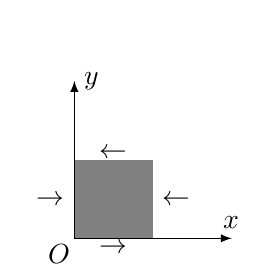
\begin{tikzpicture}[>=latex]
        \fill[color=gray](0,0)rectangle(1,1);
        \draw[->] (0,0)--(2,0)node[above]{\(x\)};
        \draw[->] (0,0)--(0,2)node[right]{\(y\)};
        \node at (-0.2,-0.2){\(O\)};
        \node at (0.5,-0.1){\(\rightarrow\)};
        \node at (0.5,1.1){\(\leftarrow\)};
        \node at (-0.3,0.5){\(\rightarrow\)};
        \node at (1.3,0.5){\(\leftarrow\)};
    \end{tikzpicture}
\end{figure}
\begin{enumerate}
    \item 最上面的箭头为\(P_{yx}<0\)
    \item 最下面的箭头为\(P_{-yx}>0\)
    \item 最右边的箭头为\(P_{xx}<0\)
    \item 最左边的箭头为\(P_{-xx}>0\)
\end{enumerate}

\section{广义牛顿黏性假设}

\subsection{牛顿黏性假设}
\begin{equation}
    \tau_{zx}=\mu\dfrac{\mathrm{d}u}{\mathrm{d}z}
\end{equation}

其中\(\mu\)为反映流体黏性的黏性系数或内摩擦系数,而流体与其他物体的黏性系数则称为外摩擦系数。牛顿黏性定律建立了黏性应力与流速分布之间的关系。

\subsection{广义牛顿黏性假设}

在牛顿黏性假设前提下假定满足三个条件
\begin{enumerate}
    \item 应力张量为形变张量的线性函数
    \item 流体为各向同性,即流体物理性质在各个方向上都相同
    \item 当流体静止时,流体中的应力为流体的静压强
\end{enumerate}

牛顿将以上的黏性应力与形变率的关系推广到任意黏性流体运动,即广义牛顿黏性假设
\begin{equation}
    P=2\mu{A}-\left(p+\dfrac{2}{3}\mu\nabla\cdot\overrightarrow{V}\right)I
\end{equation}

\(P\)为应力张量,\(A\)为形变率,\(I\)为三阶单位矩阵,\(p=\dfrac{1}{3}(p_{xx}+p_{yy}+p_{zz})\)

对于理想流体,黏性力不存在。对于不可压缩流体,散度为\(0(\nabla\cdot\overrightarrow{V}=0)\)

\section{流体的运动方程}
\begin{equation}
    \dfrac{\mathrm{d}\overrightarrow{V}}{\mathrm{d}t}=\overrightarrow{F}+\dfrac{1}{\rho}\nabla\cdot{P}
\end{equation}

将应力张量代入到运动方程中
\begin{equation}
    \dfrac{\mathrm{d}\overrightarrow{V}}{\mathrm{d}t}=\overrightarrow{F}-\dfrac{1}{\rho}\nabla{p}+\dfrac{1}{3}\dfrac{\mu}{\rho}\nabla\nabla\cdot\overrightarrow{V}+\dfrac{\mu}{\rho}\nabla^2\overrightarrow{V}
\end{equation}

这就是适合牛顿黏性假设的流体运动\(N-S\)方程。

定义\(\dfrac{\mu}{\rho}\)流体运动学黏性系数,记作\(\nu\)。

对于不可压流体\(\nabla\cdot\overrightarrow{V}=0\),方程简化为
\begin{equation}
    \dfrac{\mathrm{d}\overrightarrow{V}}{\mathrm{d}t}=\overrightarrow{F}-\dfrac{1}{\rho}\nabla{p}+\nu\nabla^2\overrightarrow{V}
\end{equation}

直角坐标系形式中(分量形式要求掌握)
\begin{equation}
\left\{
\begin{array}{c}
    \dfrac{\partial{u}}{\partial{t}}+u\dfrac{\partial{u}}{\partial{x}}+v\dfrac{\partial{u}}{\partial{y}}+w\dfrac{\partial{u}}{\partial{z}}=F_x-\dfrac{1}{\rho}\dfrac{\partial{p}}{\partial{x}}+\nu\nabla^2u\\
    \dfrac{\partial{v}}{\partial{t}}+u\dfrac{\partial{v}}{\partial{x}}+v\dfrac{\partial{v}}{\partial{y}}+w\dfrac{\partial{v}}{\partial{z}}=F_y-\dfrac{1}{\rho}\dfrac{\partial{p}}{\partial{y}}+\nu\nabla^2v\\
    \dfrac{\partial{w}}{\partial{t}}+u\dfrac{\partial{w}}{\partial{x}}+v\dfrac{\partial{w}}{\partial{y}}+w\dfrac{\partial{w}}{\partial{z}}=F_z-\dfrac{1}{\rho}\dfrac{\partial{p}}{\partial{z}}+\nu\nabla^2w\\
\end{array}
\right.
\end{equation}

牛顿第二定律在流体力学中的表示式,表明了作用力与流体运动参量之间的关系

将散度项加上\(\dfrac{u\partial}{3\rho\partial{x}}(\dfrac{\partial{u}}{\partial{x}}+\dfrac{\partial{v}}{\partial{y}}+\dfrac{\partial{w}}{\partial{z}})\)最后的黏性项为\(\nu(\dfrac{\partial^2u}{\partial{x^2}}+\dfrac{\partial^2u}{\partial{y^2}}+\dfrac{\partial^2u}{\partial{z^2}})\)
\begin{equation}
    \dfrac{\mathrm{d}\overrightarrow{V}}{\mathrm{d}t}=\overrightarrow{F}-\dfrac{1}{\rho}\nabla{p}+\nu\nabla^2\overrightarrow{V}
\end{equation}

\(\dfrac{1}{\rho}\nabla{p}\)表示压力梯度力\(\nu\nabla^2\overrightarrow{V}\)表示黏性力,黏性力不一定都是阻力,是相对运动速度而言,有可能是动力,也有可能在运动过程中不表现出来

不考虑黏性的运动方程为欧拉方程
\begin{equation}
    \dfrac{\mathrm{d}\overrightarrow{V}}{\mathrm{d}t}=\overrightarrow{F}-\dfrac{1}{\rho}\nabla{p}
\end{equation}

静力方程的公式,速度为0
\begin{equation}
    0=\overrightarrow{F}-\dfrac{1}{\rho}p
\end{equation}

可用来推导等压线方程

\section{能量方程}%好像不怎么考

了解方程各项的物理意义。

\subsection{总能量机械能和热能(内能)}

\subsection{动能和内能\(c_0T+\dfrac{1}{2}\overrightarrow{V}^2\)(单位质量)}

\subsection{质量力做功率}\begin{equation}\iiint_\tau\rho(\overrightarrow{F}\cdot\overrightarrow{V})\delta\tau\end{equation}

\subsection{表面力}
\begin{gather}
    \iint_\sigma(\overrightarrow{p}_n\cdot\overrightarrow{V})\delta\sigma\\
    \iint_\sigma(\overrightarrow{p}_n\cdot\overrightarrow{V})\delta\sigma=\iint_\sigma(\overrightarrow{n}\cdot{P}\cdot\overrightarrow{V})\delta\sigma=\iint_\sigma(P\cdot\overrightarrow{V})\delta\sigma=\iiint_\tau\nabla\cdot(P\cdot\overrightarrow{V})\delta\tau
\end{gather}

\subsection{热流入量变化率}
\begin{equation}
    \dfrac{\mathrm{d}}{\mathrm{d}t}\iiint_\tau\rho{q}\delta\tau
\end{equation}

(单位时间内从外界输入该系统单位质量流体的热流入量)

\subsection{流体系统总能量}

(内能+动能)的变化=作用于该系统上质量力和表面力对系统所做的功
\begin{equation}
    \dfrac{\mathrm{d}}{\mathrm{d}t}\iiint_\tau(c_0T+\dfrac{1}{2}\overrightarrow{V}^2)\delta\tau=\iiint_\tau\rho(\overrightarrow{F}\cdot\overrightarrow{V})\delta\tau+\iiint_\tau\nabla\cdot(P\cdot\overrightarrow{V})\delta\tau+\dfrac{\mathrm{d}}{\mathrm{d}t}\iiint_\tau\rho{q}\delta\tau\label{eqa:eg}
\end{equation}

上式\ref{eqa:eg}从左往右四项依次为:在单位时间内对流体所做的功,质量力做功率,表面力做功率,热流量的变化率

\subsection{伯努利方程}
\begin{equation}
    \dfrac{\overrightarrow{V}^2}{2}+\phi+\dfrac{p}{\rho}=const
\end{equation}

条件理想,正压,有势力,定常运动,沿流线或迹线运动

含义:理想正压流体在重力作用下作定常运动时,流体的总机械能(动能,重力势能,压力能之和)沿着流线或迹线守恒。

总结
\begin{gather}
    P=2\mu{A}-\left(p+\dfrac{2}{3}\mu\nabla\cdot\overrightarrow{V}\right)I\\
    \tau_n=2\mu{A}n-\left(\dfrac{2}{3}\mu\nabla\cdot\overrightarrow{V}\right)In\\
    \overrightarrow{p}_n=\overrightarrow{n}\cdot{P}\\
    \overrightarrow{p}_{nn}=\overrightarrow{n}\cdot\overrightarrow{p}_n
\end{gather}

\chapter{实验流体力学的基本原理和方法}

流体力学实验通常是在实验室条件下对实际流动和原型流动进行模拟。即把原型流动模拟成实验室的模型流动。原形和模型中物理过程的本质完全一致,实验室的模型流动真正能代表原形中的流动。流体力学的相似分为:几何相似,运动相似,动力相似

\section{量纲}

量纲表达了物理量的种类,是测量单位抽象化的表示式。它可以分为基本量纲和导出量纲。一个物理量均可以表示为特征值和某一无量纲数的乘积。物理量=特征值\(\times\)无量纲数。

无量纲数是以特征值为尺度所测得的该物理量的具体大小,用带撇号的小写字母表示,反映该物理量的具体大小,无量纲数总是在1左右,与单位制的选择无关,且不因单位制的改变而发生变化。

特征值随单位制所引起的物理量数值的大小变化,而在同一过程中,特征值通常是取定不变的。特征值用大写字母表示,含有量纲,反映该物理量的一般大小。

无量纲方程可以导出两个流场的相似判据对应的特征无量纲数相等。由特征无量纲数判定的相似流场只是“特征相似",不是"严格相似"。

量纲分析法\(\pi\)定理

\(\pi\)定理的主要思想利用量纲分析理论,将关系式转化为无量纲形式,减少函数中自变量的数目,从而来简化问题。

\section{相似判据}

通常可以采用两种方法来确定动力相似判据

\subsection{\(\pi\)定理方法}

是以量纲分析为基础的一种方法。

前提条件假定原型和模型流场是满足几何相似和运动相似的,考虑不可压缩黏性流体的简单情况

\subsection{方程分析法}

描述流体的运动方程反映了动力过程,也反映了各物理量之间的一种相互制约关系,从方程出发,抓住原型流动和模型流动的物理本质一致(从数学上,就要求反映原型流动和模型流动的方程同时成立),从而得到必须满足的关系式,即相似判据。

由方程推出无量纲形式

对于原型流动,考虑运动方程在z方向的分量方程
\begin{equation}
    \rho_1\dfrac{\partial{w_1}}{\partial{t_1}}+\rho\overrightarrow{V}_1\cdot\nabla_1w_1=-\rho_1g_1-\dfrac{\partial{p_1}}{\partial{z_1}}+\mu_1\nabla_1^2w_1
\end{equation}

上方程反映实际流场的动力性质和过程
\begin{equation}
    \rho_2\dfrac{\partial{w_2}}{\partial{t_2}}+\rho\overrightarrow{V}_2\cdot\nabla_2w_2=-\rho_2g_2-\dfrac{\partial{p_2}}{\partial{z_2}}+\mu_2\nabla_2^2w_2
\end{equation}

两式相比,在将比例代入有
\begin{equation}
    \dfrac{c_\rho{}c_v}{c_t}\rho_1\dfrac{\partial{w_1}}{\partial{t_1}}+\dfrac{c_\rho{}c_v^2}{c_l}\rho_1\overrightarrow{V}_1\cdot\nabla_1w_1=-c_\rho{}c_g\rho_1g_1-\dfrac{c_\rho}{c_l}\dfrac{\partial{p_1}}{\partial{z_1}}+\dfrac{c_\mu{}c_v}{c_l^2}\mu_1\nabla_1^2w_1
\end{equation}

考虑到实际流场所遵循的运动方程,只有满足
\begin{equation}
    \dfrac{c_\rho{}c_v}{c_t}=\dfrac{c_\rho{}c_v^2}{c_l}=c_\rho{}c_g=\dfrac{c_\rho}{c_l}=\dfrac{c_\mu{}c_v}{c_l^2}
\end{equation}

才能成立方程,所以得到
\begin{equation}
    \dfrac{l_1}{t_1u_1}=\dfrac{l_2}{t_2u_2},\dfrac{u_1^2}{g_1l_1}=\dfrac{u_2^2}{g_2l_2},\dfrac{p_1}{\rho_1u_1^2}=\dfrac{p_2}{\rho_2u_2^2},\dfrac{l_1u_1\rho_1}{\mu_1}=\dfrac{l_2u_2\rho_2}{\mu_2}
\end{equation}

\subsection{定义无量纲数}

\subsubsection{(特征)雷诺数\(Re\)}\begin{equation}Re=\dfrac{\text{(特征)惯性力}}{\text{(特征)黏性力}}=\dfrac{vl}{\nu}=\dfrac{UL}{\nu}\end{equation}

惯性力\(\dfrac{U^2}{L}\to{}u\dfrac{\partial{w}}{\partial{x}}\)黏性力\(\nu\dfrac{U}{L^2}\to\mu\nabla^2w\to\mu\dfrac{\partial}{\partial{x}}(\dfrac{\partial{w}}{\partial{x}})\)

\(Re\gg1\)黏性小\(Re\ll1\)强黏性\(Re\approx1\)一般黏性运动

\subsubsection{(特征)弗劳德数\(Fr\)}\begin{equation}Fr=\dfrac{\text{(特征)惯性力}}{\text{(特征)重力}}=\dfrac{v^2}{gl}=\dfrac{U^2}{gL}\end{equation}

重力\(g\to gz\)

考虑旋转时
\begin{equation}
    Fr=\dfrac{\text{(特征)旋转惯性力}}{\text{(特征)重力}}=\dfrac{\Omega^2L}{g}=\dfrac{(\Omega{L})^2/L}{g}
\end{equation}

旋转惯性力\((\Omega{L})^2/L,U=\Omega{L}\)(\(\Omega\)为旋转角动量)

\(Fr\gg1\)小尺度高速运动(航空),\(Fr\ll1\)大尺度缓慢运动

\subsubsection{斯特劳哈尔数\(Sr\)}
\begin{equation}
    Sr=\dfrac{L}{t\overrightarrow{V}}
\end{equation}

\subsubsection{欧拉数\(Eu\)}
\begin{equation}
    Eu=\dfrac{\text{压力梯度力}}{\text{惯性力项}}=\dfrac{\Delta{P}}{\rho{\overrightarrow{V}}^2}
\end{equation}

\subsubsection{罗斯贝数\(Ro\)衡量旋转效应}
\begin{equation}
    Ro=\dfrac{\text{特征惯性力}}{\text{特征偏向力}}=\dfrac{U}{\Omega{L}}=\dfrac{U^2/L}{\Omega{U}}
\end{equation}

总结:无量纲数较为重要的为雷诺数,弗劳德数,定义需要记忆,这两个为特征惯性力/特征黏性力或特征重力,惯性力和黏性力的公式记住,再对公式进行无量纲分析,得出结论。

以雷诺数为例,当它远远小于1时,说明黏性力重要,不能忽略,反之,即不重要。

\chapter{流体涡旋动力学基础}

\section{环流的起源}

流体涡度它是反应流体旋转特征或者旋转强度的一个重要物理量。涡度为零时,流体运动为无旋的,涡度不等于零时,则对应流体的涡旋运动。

在流场中任取一个封闭的物质环线\(l\)(形状大小可变,由流点组成的闭合曲线)。

速度环流的定义\(\Gamma=\oint_l\overrightarrow{V}\cdot\mathrm{d}\overrightarrow{l}\)它反应了流体沿曲线\(l\)运动的趋势,是标量,但具有一定的方向性。

如取定曲线方向\(\Gamma>0\)流体有顺\(\overrightarrow{l}\)运动的趋势(逆时针为正方向,对应气旋环流)。\(\Gamma<0\)流体有逆\(\overrightarrow{l}\)运动的趋势(顺时针为负方向,对应反气旋环流)。

\subsection{开尔文定理(速度环流的守恒定律)}

\subsubsection{环流的变化(环流加速度)}
\begin{gather}
    \dfrac{\mathrm{d}\Gamma}{\mathrm{d}t}=\dfrac{\mathrm{d}}{\mathrm{d}t}\oint_l\overrightarrow{V}\cdot\delta\overrightarrow{l}=\oint_l\dfrac{\mathrm{d}\overrightarrow{V}}{\mathrm{d}t}\cdot\delta\overrightarrow{l}+\oint_l\overrightarrow{V}\dfrac{\mathrm{d}(\delta\overrightarrow{l})}{\mathrm{d}t}\\
    \oint_l\overrightarrow{V}\dfrac{\mathrm{d}(\delta\overrightarrow{l})}{\mathrm{d}t}=\oint_l\overrightarrow{V}\cdot\delta\overrightarrow{V}=\oint_l\delta\left(\dfrac{\overrightarrow{V}^2}{2}\right)=0
\end{gather}

所以
\begin{equation}
    \dfrac{\mathrm{d}\Gamma}{\mathrm{d}t}=\oint_l\dfrac{\mathrm{d}\overrightarrow{V}}{\mathrm{d}t}\cdot\delta\overrightarrow{l}
\end{equation}

环流加速度=加速度的环流

\subsubsection{流体的正压性和斜压性}

流体分为正压流体和斜压流体两类

对于正压流体,密度仅是压力的函数,即等压面,等密度面,等温面重合

对于斜压流体,密度不仅与压力有关,还与其他参数有关,如温度,湿度等
\begin{enumerate}
    \item 理想流体运动方程(欧拉方程)\(\dfrac{\mathrm{d}\overrightarrow{V}}{\mathrm{d}t}=\overrightarrow{F}-\dfrac{1}{\rho}\nabla{p}\)
    \item 质量力仅为有势力\(F=-\nabla\Phi\)
    \item 正压流体\(\rho=f(p)\)等压面,等密度面,等温面重合。有\(\dfrac{\mathrm{d}\Gamma}{\mathrm{d}t}=\)或\(\Gamma=const\)
\end{enumerate}

理想正压流体,在有势力的作用下,速度环流不随时间变化,这就是开尔文环流定理。

\subsubsection{普遍情况下的环流变化表达式}

对于对于黏性可压缩流体,运动方程为
\begin{equation}
    \dfrac{\mathrm{d}\overrightarrow{V}}{\mathrm{d}t}=\overrightarrow{F}-\dfrac{1}{\rho}\nabla{p}+\nu\nabla^2\overrightarrow{V}+\dfrac{\nu}{3}\nabla(\nabla\cdot\overrightarrow{V})
\end{equation}

然后对上式中黏性扩散项进行处理(矢量运算法则),得到
\begin{equation}
    \dfrac{\mathrm{d}\overrightarrow{V}}{\mathrm{d}t}=\overrightarrow{F}-\dfrac{1}{\rho}\nabla{p}+\nu\left(\dfrac{4}{3}\nabla{D}-\nabla\times\overrightarrow{\zeta}\right)
\end{equation}

对上式沿闭合曲线进行积分,即可得到反映环流变化的方程
\begin{equation}
    \dfrac{\mathrm{d}\Gamma}{\mathrm{d}t}=\oint_l\dfrac{\mathrm{d}\overrightarrow{V}}{\mathrm{d}t}\cdot\delta\overrightarrow{l}=\oint_l\overrightarrow{F}\cdot\delta\overrightarrow{l}-\oint_l\dfrac{1}{\rho}\nabla{p}\cdot\delta\overrightarrow{l}-\nu\oint_l\nabla\times\overrightarrow{\zeta}\cdot\delta\overrightarrow{l}
\end{equation}

\subsubsection{速度环流的变化,主要由以下3项所引起}
\begin{enumerate}
    \item 非有势力的作用
    \item 压力--密度或压力梯度力
    \item 黏性涡度扩散
\end{enumerate}

\subsection{皮耶克尼斯定理}

理想斜压流体在有势力的作用下,斜压性可引起速度环流发生变化。进一步讨论环流方程斜压流体(主要是斜压项的讨论及应用),将线积分转化为面积分,则有
\begin{equation}
    \begin{aligned}
    -\oint_l\dfrac{1}{\rho}\nabla{p}\cdot\delta\overrightarrow{l}&=-\iint_\sigma\nabla\times(\dfrac{\nabla{p}}{\rho})\cdot\delta\overrightarrow{\sigma}\\
    &=-\iint_\sigma[\nabla(\dfrac{1}{\rho})\times\nabla{p}+\dfrac{1}{\rho}\nabla\times(\nabla{p})]\delta\overrightarrow{\sigma}\\
    &=-\iint_\sigma[\nabla(\dfrac{1}{\rho})\times\nabla{p}]\delta\overrightarrow{\sigma}
    \end{aligned}
\end{equation}

(\(\dfrac{1}{\rho}\nabla\times(\nabla{p})\)的旋度为0)若作理想流体假设,且外力有势,则环流定理变为皮耶克尼斯定理
\begin{equation}
    \dfrac{\mathrm{d}\Gamma}{\mathrm{d}t}=-\oiint_\sigma[\nabla(\dfrac{1}{\rho})\times\nabla{p}]\cdot\delta\overrightarrow{\sigma}
\end{equation}

反映了压力--密度项(斜压性)引起环流的变化取决于等密度面或者等比容面与等压面是否斜交。可以用来解释海陆风,山谷风以及环流的形成原理

例:
\begin{figure}[h!]
    \centering
    \begin{minipage}{0.4\linewidth}
        \centering
        \caption{白天海陆风}
        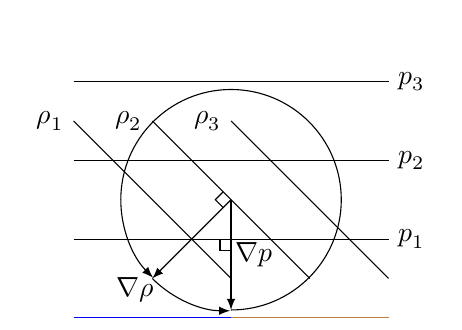
\begin{tikzpicture}[>=latex]
            \draw[blue] (-2,0)--node[below]{海洋}(0,0);
            \draw[brown] (0,0)--node[below]{陆地}(2,0);
            \foreach \y in {1,2,3}{
                \draw (-2,\y)--(2,\y)node[right]{\(p_\y\)};
            }
            \draw (-2,2.5)node[left]{\(\rho_1\)}--(0,0.5);
            \draw (-1,2.5)node[left]{\(\rho_2\)}--(1,0.5);
            \draw (0,2.5)node[left]{\(\rho_3\)}--(2,0.5);
            \draw[->] (0,1.5)--(-1,0.5)node[below left=-4pt]{\(\nabla\rho\)};
            \draw[->] (0,1.5)--node[right=-2pt]{\(\nabla p\)}(0,0.1);
            \draw (-0.1,1.4)--(-0.2,1.5)--(-0.1,1.6);
            \draw (0,0.86)-|(-0.14,1);
            \draw[->] (-1,0.5) arc [start angle=225,end angle=270,radius=1.4cm];
            \draw[->] (0,0.1) arc [start angle=-90,end angle=225,radius=1.4cm];
        \end{tikzpicture}
    \end{minipage}
    \begin{minipage}{0.4\linewidth}
        \centering
        \caption{夜晚海陆风}
        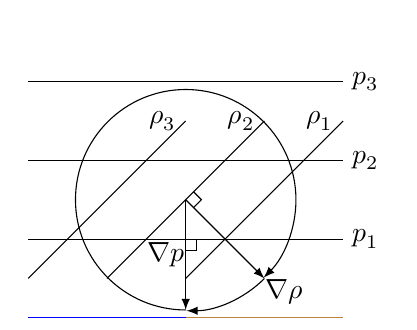
\begin{tikzpicture}[>=latex]
            \draw[blue] (-2,0)--node[below]{海洋}(0,0);
            \draw[brown] (0,0)--node[below]{陆地}(2,0);
            \foreach \y in {1,2,3}{
                \draw (-2,\y)--(2,\y)node[right]{\(p_\y\)};
            }
            \draw (2,2.5)node[left]{\(\rho_1\)}--(0,0.5);
            \draw (1,2.5)node[left]{\(\rho_2\)}--(-1,0.5);
            \draw (0,2.5)node[left]{\(\rho_3\)}--(-2,0.5);
            \draw[->] (0,1.5)--(1,0.5)node[below right=-3pt]{\(\nabla\rho\)};
            \draw[->] (0,1.5)--node[left=-3pt]{\(\nabla p\)}(0,0.1);
            \draw (0.1,1.4)--(0.2,1.5)--(0.1,1.6);
            \draw (0,0.86)-|(0.14,1);
            \draw[->] (1,0.5) arc [start angle=315,end angle=270,radius=1.4cm];
            \draw[->] (0,0.1) arc [start angle=270,end angle=-45,radius=1.4cm];
        \end{tikzpicture}
    \end{minipage}
\end{figure}

此处均有\(p_1>p_2>p_3,\rho_1>\rho_2>\rho_3\)

\subsection{涡度方程}
\begin{equation}
    \dfrac{\mathrm{d}\overrightarrow{\zeta}}{\mathrm{d}t}=\dfrac{1}{\rho^2}\nabla\rho\times\nabla{p}-\overrightarrow{\zeta}(\nabla\cdot\overrightarrow{V})+(\overrightarrow{\zeta}\cdot\nabla)\overrightarrow{V}+\nu\nabla^2\overrightarrow{\zeta}
\end{equation}

\subsubsection{力管项或斜压项}

它表明了压力--密度变化可以引起流体涡度矢的变化,其物理实质是流体的斜压性。

\subsubsection{散度项}

它表明了流体在运动过程中体积的收缩或膨胀,将会引起流体涡度矢的变化。

可以类比于花样滑冰运动员,当身体伸展开始,旋转速度减慢,收缩时,旋转速度增加。

\subsubsection{扭曲项}

表明流场的非均匀性会引起涡度矢发生改变。扭曲项并不改变涡旋的强度,只是使涡度矢在三个方向上重新分布。

\subsubsection{黏性扩散项}

涡度分布的非均匀性引起的。涡旋强的地方将向涡旋弱的地方输送涡旋,直到涡旋强度相等为止。

\subsection{总结}

真正直接产生流体质点涡度矢的主要有流体的斜压性,非有势力和流体的黏性。

\chapter{流体波动}

\section{波参数}
\begin{equation}
    y=A\cos(kx-\omega{t}+\varphi)=A\cos{}[k(x-ct)]
\end{equation}

\subsection{波长\(L\)}

固定\(t\)相邻同相位之间的距离
\begin{figure}[htbp]
    \centering
    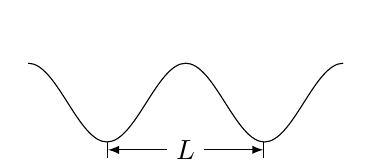
\begin{tikzpicture}[>=latex,scale=0.5]
        \draw (0,1) cos (1,0) sin (2,-1) cos (3,0) sin (4,1) cos (5,0) sin (6,-1) cos (7,0) sin (8,1);
        \draw[|<->|] (2,-1.2)--node[fill=white]{\(L\)}(6,-1.2);
    \end{tikzpicture}
\end{figure}

\subsection{位相}
\begin{equation}
    \theta=kx-\omega{t}+\varphi
    \rightarrow
    \left\{
    \begin{array}{c}
    \text{平面(平波面)}\\
    \text{球面(球波面)}
    \end{array}
    \right.
\end{equation}

\subsection{波数}
\begin{equation}
    k=\dfrac{2\pi}{L}
\end{equation}

\subsection{圆频率}
\begin{equation}
    \omega=\dfrac{2\pi}{T}
\end{equation}

\subsection{相速}
\begin{equation}
    c=\dfrac{\omega}{k}=\dfrac{L}{T}
\end{equation}

速度矢量\(c\)不具有运动速度矢量的特点

\section{水面重力波(微小扰动)}

要求会推导水面重力波,理解波动机制。
\begin{equation}
    h'(x_1,t)=h(x_1,t)-H
\end{equation}

\(H\)平均平静时的不考虑黏性的不可压缩流体
\begin{equation}
    \begin{cases}
    \dfrac{\mathrm{d}u}{\mathrm{d}t}=-\dfrac{1}{\rho}\dfrac{\mathrm{d}p}{\mathrm{d}x}\\
    \dfrac{\partial{h}}{\partial{t}}+u\dfrac{\partial{h}}{\partial{x}}+h\dfrac{\partial{u}}{\partial{x}}=0\text{(自由表面的流体连续方程)}
    \end{cases}
    \label{eqa2}
\end{equation}

由
\begin{equation}
    P=P_0+\rho{g}[h(x,H-z)]
\end{equation}

对\(x\)求偏导
\begin{equation}
    \dfrac{1}{\rho}\dfrac{\partial{p}}{\partial{x}}=g\dfrac{\partial{h}}{\partial{x}}
    \label{eqa3}
\end{equation}

将其带入式\ref{eqa2}
\begin{equation}
    \begin{cases}
    \dfrac{\partial{u}}{\partial{t}}+\overrightarrow{V}\cdot\nabla{u}=-g\dfrac{\partial{h}}{\partial{x}}\\
    \dfrac{\partial{h}}{\partial{t}}+u\dfrac{\partial{h}}{\partial{x}}+h\dfrac{\partial{u}}{\partial{x}}=0
    \end{cases}
    \label{eqa4}
\end{equation}

又
\begin{equation}
    \begin{cases}
    v=0\\
    \dfrac{\partial}{\partial{y}}=0
    \end{cases}
\end{equation}

代入式\ref{eqa4}得
\begin{equation}
    \begin{cases}
    \dfrac{\partial{u}}{\partial{t}}+u\dfrac{\partial{u}}{\partial{x}}+w\dfrac{\partial{u}}{\partial{z}}=-g\dfrac{\partial{h}}{\partial{x}}\\
    \dfrac{\partial{h}}{\partial{t}}+u\dfrac{\partial{h}}{\partial{x}}+h\dfrac{\partial{u}}{\partial{x}}=0
    \end{cases}
    \label{eqa5}
\end{equation}

化为线性
\begin{equation}
    u=\bar{u}+u',h=H+h',w=\bar{w}+w'
\end{equation}

代入式\ref{eqa5}得

基本态\(\bar{u}=0\)
\begin{equation}
    \left\{
        \begin{array}{l}
        \dfrac{\partial{\bar{u}}}{\partial{t}}+\bar{u}\dfrac{\partial{\bar{u}}}{\partial{x}}+\bar{w}\dfrac{\partial{\bar{w}}}{\partial{z}}=-g\dfrac{\partial{H}}{\partial{x}}=0\\
        \dfrac{\partial{H}}{\partial{t}}=-\bar{u}\dfrac{\partial{H}}{\partial{x}}-H\dfrac{\partial\bar{u}}{\partial{x}}=0
        \end{array}
    \right.
    \left\{
        \begin{array}{l}
        \dfrac{\partial{u}'}{\partial{t}}+u'\dfrac{\partial{u}'}{\partial{x}}+w'\dfrac{\partial{u}'}{\partial{z}}=-g\dfrac{\partial{h}'}{\partial{x}}\\
        \dfrac{\partial{h}'}{\partial{t}}+u'\dfrac{\partial{h}'}{\partial{x}}+(H+h')\dfrac{\partial{u}'}{\partial{x}}=0
        \end{array}
    \right.
    \label{eqa6}
\end{equation}

化简得
\begin{align}
    \dfrac{\partial{u}'}{\partial{t}}=-g\dfrac{\partial{h}'}{\partial{x}} \label{eqa7}\\
    \dfrac{\partial{h}'}{\partial{t}}=-H\dfrac{\partial{u}'}{\partial{x}} \label{eqa8}
\end{align}

消去含\(u\)的项--式\ref{eqa8}对\(t\)求偏导后乘以\(H+\)式\ref{eqa7}对\(x\)求偏导得 
\begin{equation}
    \dfrac{\partial^2h'}{\partial{t}^2}=gH\dfrac{\partial^2h'}{\partial{x}^2}
\end{equation}

假设\(h'(x,t)=A\sin{}[k(x-ct)]\)代入得
\begin{equation}
    c=\pm\sqrt{gH}
\end{equation}

即\(h'(x,t)=A\sin{}[k(x\pm\sqrt{gH}t)]\) 

假设\(u'(x,t)=B\sin{}[k(x-ct)]\)
\begin{equation}
    u'(x,t)=B\sin{}[k(x-ct)]=\pm\sqrt{\dfrac{g}{H}}A\sin{}[k(x-ct)]
\end{equation}

振动机制水面受到外界干扰后\((\dfrac{\partial{h}'}{\partial{x}}\neq0)\),重力作用产生水平压力梯度力\((-g\dfrac{\partial{h}'}{\partial{x}}\neq0)\),引起运动\((\dfrac{\partial{u}'}{\partial{t}}\neq0)\),流动结果会出现水平辐合辐散\((\dfrac{\partial{u}'}{\partial{x}}\neq0)\),最后改变了原来水面的起伏\((\dfrac{\partial{h}'}{\partial{t}}\neq0)\)

\section{上轻下重流体间的界面波}

\((\rho1<\rho2)\)
\begin{figure}[htbp]
    \centering%教材上大致是这样的?
    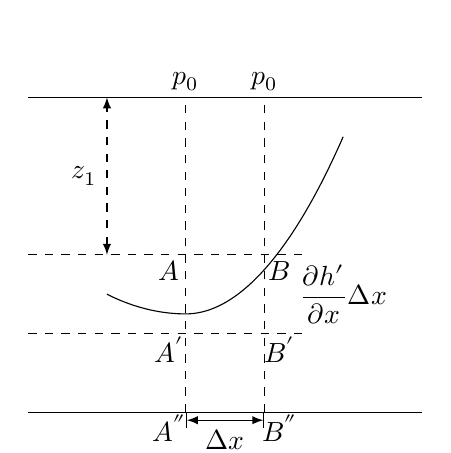
\begin{tikzpicture}[>=latex]
        \foreach \y/\n/\m in {0/{}/5,1/{dashed}/3.5,2/{dashed}/3.5,4/{}/5}
        {
            \draw[\n] (0,\y)--(\m,\y);
        }
        \foreach \x in {2,3}
        {
            \draw[dashed] (\x,0)--(\x,4);
        }
        \draw[dashed,<->] (1,2)--node[left]{\(z_1\)}(1,4);
        \foreach \a/\b in {{}/1.8,{'}/0.8,{''}/-0.2}
        {
            \node at (1.8,\b){\(A^{\a}\)};
            \node at (3.2,\b){\(B^{\a}\)};
        }
        \node at (2,4.2){\(p_0\)};
        \node at (3,4.2){\(p_0\)};
        \node at (4,1.5){\(\dfrac{\partial h'}{\partial x}\Delta x\)};
        \draw[|<->|](2,-0.1)--node[below]{\(\Delta x\)}(3,-0.1);
        \draw (1,1.5) parabola bend (2,1.25) (4,3.5);
    \end{tikzpicture}
\end{figure}

选择下层流体作为研究对象
\begin{equation}
    \begin{cases}
    \dfrac{\mathrm{d}u}{\mathrm{d}t}=-\dfrac{1}{\rho_2}\dfrac{\mathrm{d}p}{\mathrm{d}x}\\
    \dfrac{\partial{h}}{\partial{t}}+u\dfrac{\partial{h}}{\partial{x}}+h\dfrac{\partial{u}}{\partial{x}}=0
    \end{cases}
    \label{eqa9}
\end{equation}

\(P_A=P_B=P_0+\rho_1gz_1\)

由\(\dfrac{\partial{P}}{\partial{z}}=-\rho{g}\)可推出,对于不可压缩流体有\(\dfrac{\partial}{\partial{x}}\left(\dfrac{\partial{p}}{\partial{z}}\right)=0\)或\(\dfrac{\partial}{\partial{z}}\left(\dfrac{\partial{p}}{\partial{x}}\right)=0\)

即\(-\dfrac{1}{\rho}\dfrac{\partial{p}}{\partial{x}}\)不随高度\(z\)变化
\begin{align}
    -\dfrac{1}{\rho_2}\dfrac{\partial{p}}{\partial{x}}=-\dfrac{1}{\rho_2}\lim_{\Delta{x}\to0}\dfrac{1}{\Delta{x}}(p_B''-p_A'')=-\dfrac{1}{\rho_2}\lim_{\Delta{x}\to0}\dfrac{1}{\Delta{x}}(p_B'-p_A')\label{eqa10}\\
    P_A'=P_A+\left(\dfrac{\partial{h'}}{\partial{t}}\Delta{x}\right)\rho_1g=P+\left(\dfrac{\partial{h'}}{\partial{x}}\Delta{x}\right)\rho_1g\label{eqa11}\\
    P_B'=P_B+\left(\dfrac{\partial{h'}}{\partial{t}}\Delta{x}\right)\rho_2g=P+\left(\dfrac{\partial{h'}}{\partial{x}}\Delta{x}\right)\rho_2g\label{eqa12}
\end{align}

把式\ref{eqa11},式\ref{eqa12}代入式\ref{eqa10}得
\begin{equation}
    -\dfrac{1}{\rho_2}\dfrac{\partial{p}}{\partial{x}}=-g\left(1-\dfrac{\rho_1}{\rho_2}\right)\dfrac{\partial{h}}{\partial{x}}\label{eqa13}
\end{equation}

把式\ref{eqa13}代入式\ref{eqa9}得
\begin{equation}
    \begin{cases}
    \dfrac{\partial{u}}{\partial{x}}+u\dfrac{\partial{u}}{\partial{x}}+w\dfrac{\partial{u}}{\partial{z}}=-g\left(1-\dfrac{\rho_1}{\rho_2}\right)\dfrac{\partial{h}}{\partial{x}}\\
    \dfrac{\partial{h}}{\partial{t}}+u\dfrac{\partial{h}}{\partial{x}}+h\dfrac{\partial{u}}{\partial{x}}=0
    \end{cases}
\end{equation}

化为线性
\begin{equation}
    u=\bar{u}+u',h=\bar{h}+h',w=\bar{w}+w'
\end{equation}

带入式\ref{eqa12}得基本态
\begin{equation}
    \bar{u}=0
\end{equation}

化简得
\begin{align}
    \dfrac{\partial{u'}}{\partial{t}} =& -g\left(1-\dfrac{\rho_1}{\rho_2}\right)\dfrac{\partial{h'}}{\partial{x}} \label{111}\\
    \dfrac{\partial{h'}}{\partial{t}} =& -h\dfrac{\partial{u}}{\partial{x}} \label{222}
\end{align}

消去含\(u\)的项--对式\ref{222}求\(t\)偏导\(+\)式\ref{111}对\(x\)求偏导得
\begin{equation}
    \dfrac{\partial^2h'}{\partial{t^2}}=gH\left(1-\dfrac{\rho_1}{\rho_2}\right)\dfrac{\partial^2h'}{\partial{x^2}}
\end{equation}

假设\(h'(x,t)=A\sin{}[k(x-ct)]\)代入得
\begin{equation}
    c=\pm\sqrt{gH\left(1-\dfrac{\rho_1}{\rho_2}\right)}
\end{equation}

修正重力\(g'=g\left(1-\dfrac{\rho_1}{\rho_2}\right)\)
\begin{figure}[htbp]
    \centering%?不太清楚该怎么画
    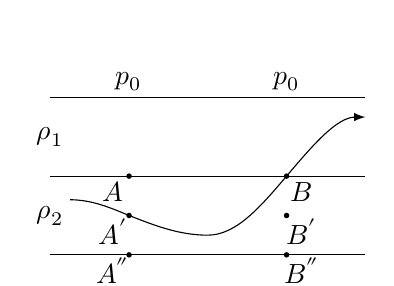
\begin{tikzpicture}[>=latex]
        \foreach \y in {0,1,2}
        {
            \draw (0,\y)--(4,\y);
        }
        \foreach \a/\b in {{}/1,{'}/0.5,{''}/0}
        {
            \node at (0.8,\b-0.2){\(A^{\a}\)};
            \node at (3.2,\b-0.2){\(B^{\a}\)};
            \fill (1,\b) circle (1pt);
            \fill (3,\b) circle (1pt);
        }
        \node at (1,2.2){\(p_0\)};
        \node at (3,2.2){\(p_0\)};
        \node at (0,0.5){\(\rho_2\)};
        \node at (0,1.5){\(\rho_1\)};
        \draw[->] (0.25,0.7) cos (1,0.5) sin (2,0.25) cos (3,1) sin (4,1.75);
    \end{tikzpicture}
\end{figure}
\(P_A=P_B=P_0+\rho_1gz_1\)

未受移动前\(\dfrac{\partial{P}}{\partial{z}}=-\rho{g},\dfrac{\partial}{\partial{x}}(\dfrac{\partial{p}}{\partial{t}})=0\),即\(\dfrac{\partial{P}}{\partial{x}}(\dfrac{\partial{p}}{\partial{t}})=0,P_B''-P_A''=P_B-P_A\)
\begin{align}
    -\dfrac{1}{\rho_2}\dfrac{\partial{p}}{\partial{x}}=-\dfrac{1}{\rho_2}\lim_{\Delta{x}\to0}\dfrac{1}{\Delta{x}}(p_B''-p_A'')=-\dfrac{1}{\rho_2}\lim_{\Delta{x}\to0}\dfrac{1}{\Delta{x}}(p_B'-p_A')\label{3}\\
    P_A'=P_A+\left(\dfrac{\partial{h'}}{\partial{t}}\Delta{x}\right)\rho_1g=P+\left(\dfrac{\partial{h'}}{\partial{x}}\Delta{x}\right)\rho_1g\label{4}\\
    P_B'=P_B+\left(\dfrac{\partial{h'}}{\partial{t}}\Delta{x}\right)\rho_2g=P+\left(\dfrac{\partial{h'}}{\partial{x}}\Delta{x}\right)\rho_2g\label{5}
\end{align}

把式\ref{4},式\ref{5}代入式\ref{3}得
\begin{equation}
    -\dfrac{1}{\rho_2}\dfrac{\partial{p}}{\partial{x}}=-g\left(1-\dfrac{\rho_1}{\rho_2}\right)\dfrac{\partial{h}}{\partial{x}}
\end{equation}

总结:上轻下重的界面波记住结论,最好会推导,推导过程与上面基本相同,就是多个证明过程

\chapter{旋转流体动力学}

\section{速度推导加入旋转惯性项}
\begin{gather}
    \dfrac{\mathrm{d}_a\overrightarrow{V}_a}{\mathrm{d}t}=\dfrac{\mathrm{d}_r\overrightarrow{V}_a}{\mathrm{d}t}+\Omega\times{}\overrightarrow{V}_a\\
    \dfrac{\mathrm{d}_a\overrightarrow{V}_a}{\mathrm{d}t}=\dfrac{\mathrm{d}_r(\overrightarrow{V}+\Omega\times{}r)}{\mathrm{d}t}+\Omega\times(\overrightarrow{V}+\Omega\times{}r)\\
    \dfrac{\mathrm{d}_a\overrightarrow{V}_a}{\mathrm{d}t}=\dfrac{\mathrm{d}_r\overrightarrow{V}}{\mathrm{d}t}+2\Omega\times{}\overrightarrow{V}+\Omega\times\Omega\times{r}=\dfrac{\mathrm{d}_r\overrightarrow{V}}{\mathrm{d}t}+2\Omega\times{}\overrightarrow{V}-\Omega^2\times{R}\\
    \dfrac{\mathrm{d}_a\overrightarrow{V}_a}{\mathrm{d}t}=-\dfrac{1}{\rho}\nabla{P}+\nu\nabla^2\overrightarrow{V}+F\\
    \dfrac{\mathrm{d}_r\overrightarrow{V}}{\mathrm{d}t}=-\dfrac{1}{\rho}\nabla{P}+\nu\nabla^2\overrightarrow{V}+F+2\Omega\times{}\overrightarrow{V}-\Omega^2\times{R}
\end{gather}

普鲁德曼--泰勒定理:不可压或者正压流体,在有势力作用下的准定常缓慢运动,由于强旋转效应,其速度与垂直坐标无关,流动趋于二维化(流动是水平二维的)。

\section{罗斯贝数衡量旋转效应}
\begin{equation}
    Ro=\dfrac{\text{特征惯性力}}{\text{特征偏向力}}=\dfrac{U^2/L}{\Omega{U}}=\dfrac{U}{\Omega{L}}
\end{equation}

惯性力\(\dfrac{U^2}{L}\to{}u\dfrac{\partial{w}}{\partial{x}}\) 偏向力\(\Omega U\to f=-2\overrightarrow{\Omega}\times\overrightarrow{V}\)

埃克曼系数\(E_k\)
\begin{equation}
    E_k=\dfrac{\text{特征黏性力}}{\text{特征偏向力}}=\dfrac{\nu}{\Omega{L^2}}=\dfrac{\nu{}U/L^2}{\Omega{U}}=\dfrac{Ro}{Re}
\end{equation}

黏性力\(\nu\dfrac{U}{L^2}\to\nu\nabla^2w\to\nu\dfrac{\partial}{\partial{x}}(\dfrac{\partial{w}}{\partial{x}})\)

\section{科氏力方向的判断(右手螺旋定则)}
\begin{gather}
    f=-2\overrightarrow{\Omega}\times\overrightarrow{V}\\
    \begin{pmatrix}
        \overrightarrow{i}&\overrightarrow{j}&\overrightarrow{k}\\
        0&\Omega\cos{}\alpha &\Omega\sin{}\alpha \\
        u&v&w\\
    \end{pmatrix}
    =-2[\Omega\cos{}(\alpha w)-\Omega\sin{}(\alpha v)]\overrightarrow{i}-2[\Omega\sin{}(\alpha u)]\overrightarrow{j}-2[-\Omega\cos{}(\alpha u)]\overrightarrow{k}\\
    -\dfrac{1}{\rho}\nabla{P}=f+\overrightarrow{g}=-2\Omega\times\overrightarrow{v}+\overrightarrow{g}\\
    \left\{
        \begin{array}{c}
        \dfrac{1}{\rho}\dfrac{\partial{P}}{\partial{x}}=2[\xcancel{-\Omega\cos{}(\alpha w)}+\Omega\sin{}(\alpha v)](w\text{是小量,可忽略})\\
        \dfrac{1}{\rho}\dfrac{\partial{P}}{\partial{y}}=-2\Omega\sin{}(\alpha u)\\
        \dfrac{1}{\rho}\dfrac{\partial{P}}{\partial{z}}=-g\xcancel{-2\Omega\cos{}(\alpha u)}(\text{相对小可以忽略})
        \end{array}\right.\\
\end{gather}

令\(f=2\Omega\sin{}\alpha\),化简得
\begin{equation}
    \begin{cases}
    \dfrac{\partial{P}}{\partial{x}}=\rho fv\\
    \dfrac{\partial{P}}{\partial{y}}=-\rho fu\\
    \dfrac{\partial{P}}{\partial{z}}=-\rho g
    \end{cases}
\end{equation}

\end{document}